Potenssifunktiossa $f(x) = x^n$ muuttuja $x$ on kantalukuna. Jos muuttuja $x$ on sen sijaan eksponenttina, saadaan joukko funktioita, joita kutsutaan \termi{eksponenttifunktio}{eksponenttifunktioiksi}.

\laatikko[Eksponenttifunktio]{Eksponenttifunktiot ovat muotoa $f(x) = a^x$, $a > 0$, $a \neq 1$ olevia funktioita.}

Funktio $f(x) = 1^x = 1$ on vakiofunktio, joten sitä ei yleensä ole järkevää tarkastella eksponenttifunktiona. Eksponenttifunktioita on kahta tyyppiä: kasvavia ja väheneviä. Kasvavilla eksponenttifunktioilla $a>1$, esimerkiksi

\begin{center}
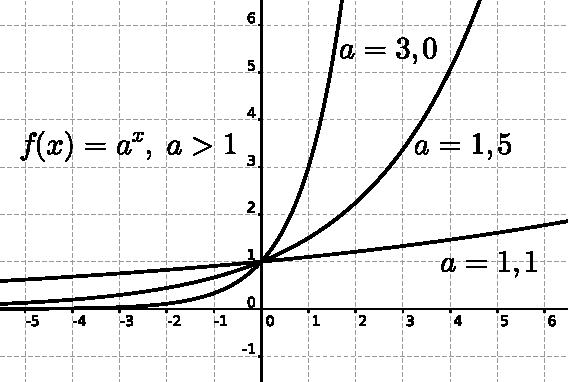
\includegraphics{pictures/apotenssiinxaisompikuinyksi.pdf}
\end{center}

Kun $a$ on pieni mutta positiivinen –  $0<a<1$, eksponenttifunktio on vähenevä:

\begin{center}
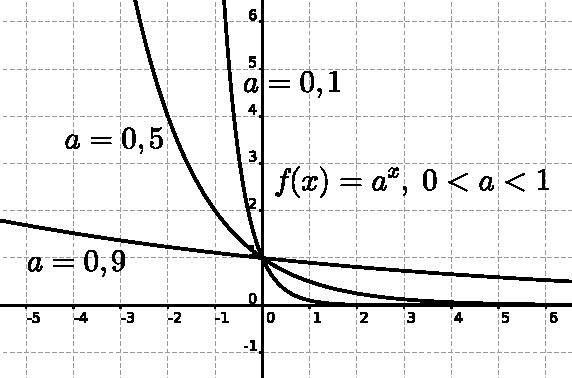
\includegraphics{pictures/apotenssiinxaisompikuinnolla.pdf}
\end{center}

Huomaa, että eksponenttifunktion kuvaaja kulkee aina pisteen $(0,1)$ kautta. Tämä johtuu potenssin laskusäännöstä, jonka mukaan $a^0=1$, kun $a\neq0$
%lisä'nnyt Jaakko Viertiö 14.12.2013

Negatiiviselle kantaluvulle ei ole määritelty yleistä reaalilukupotenssia, joten eksponenttifunktiota ei ole määritelty, kun $a < 0$. 

Kun $a=0$ tai $a=1$, eksponenttifunktio pelkistyy vakiofunktioksi. Lisäksi $0^0$:a ei ole määritelty, joten vaaditaan, että eksponenttifunktion kantaluvulle $a$ pätee $a>0$ ja $a \neq 1$.

\termi{eksponenttiyhtälö}{Eksponenttiyhtälö} muodostuu, kun kysytään, millä $x$:n arvoilla %eksponenttifunktio saavuttaa tietyn arvon.

\begin{esimerkki}
Millä muuttujan $x$ arvoilla eksponenttifunktio $f(x) = 2^x$ saa arvon$f(x) = 64$?
	\begin{esimratk}
Kirjoitetaan tehtävä yhtälöksi: $2^x = 64$. Kokeilemalla luvun $2$ potensseja huomataan, että $x = 6$ ratkaisee yhtälön.

Varmistutaan vielä siitä, että yhtälöllä ei ole muita ratkaisuja. Eksponenttifunktion kantalukuna on $2$, joten eksponenttifunktio on kasvava. Funktio $f(x) = 2^x$ ei siis voi saada uudelleen arvoa $64$, kun $x > 6$. Samasta syystä $f(x)$ ei voi olla $64$, kun $x < 6$.

Ainoa ratkaisu yhtälölle on siis $x = 6$.
	\end{esimratk}
\end{esimerkki}

\begin{esimerkki}
Millä muuttujan $x$ arvoilla eksponenttifunktio $f(x) = \left( \frac{1}{2} \right)^x$ saa arvon $f(x) = 1/5$?

	\begin{esimratk}
Edellisen esimerkin tavoin kokeillaan $x$:n eri arvoja. Havaitaan, että kun $x = 2$, funktio saa arvon $f(x) = \frac{1}{4}$, ja kun $x = 3$, on $f(x) = \frac{1}{8}$. Ratkaisu on siis välillä $2 < x < 3$.

Ratkaisun etsimistä voidaan jatkaa kokeilemalla esimerkiksi arvoa $x = 2,5$. Näin päästään lähemmäksi ratkaisua, mutta yhtälön ratkaisu on irrationaalinen, joten sen desimaalikehitelmä on äärettömän pitkä ja jaksoton. Tarkkaa ratkaisua ei siis saada tällä menetelmällä.
	\end{esimratk}
\end{esimerkki}

Yleisen eksponenttiyhtälön tarkkaan ratkaisemiseen niin sanotun logaritmin avulla palataan kurssilla MAA8. %kurssiviittausympäristö?

\subsection{Eksponentiaalinen malli}

Kun eksponenttifunktiota käytetään kuvaamaan jotakin reaalimaailman ilmiötä, siitä käytetään nimeä \termi{eksponentiaalinen malli}{eksponentiaalinen malli}.

Eksponentiaalinen malli on eräs yleisimmin käytetyistä matemaattisista malleista. Sillä kuvataan sellaista kasvua tai vähenemistä, jossa kullakin ajanhetkellä funktion hetkellinen muutos on suoraan verrannollinen funktion sen hetkiseen arvoon. Tämä muotoillaan täsmällisesti myöhemmillä matematiikan kursseilla.

\begin{esimerkki}
Soluviljelmässä olevien \textit{Escherichia coli} -bakteerien määrää voidaan kuvata eksponentiaalisella mallilla: ajanhetkellä $t = 0$ bakteerien lukumäärä on $1$, ja kullakin aika-askeleella bakteerien lukumäärä tuplaantuu. Malli voidaan kirjoittaa %ajanhetkellä yhdyssana?
\[
f(t) = 2^t, t \ge 0,
\]
jossa $f(t)$ on bakteerien lukumäärä ajanhetkellä $t$. (Tässä ei oteta kantaa käytettyyn ajan yksikköön -- mikä tahansa käy.)

Huomaa, että funktion $f(t)$ arvot voivat olla myös rationaalisia tai irrationaalisia, vaikka bakteerien määrä on kokonaisluku. Yleensä tätä ei pidetä ongelmallisena, vaan funktiota voidaan käsitellä, ikään kuin bakteerien määrä olisi jatkuvasti kasvava suure. Mallit ovat harvoin täydellisiä, eikä virhe ei ole käytännössä merkittävä, koska mallin antamat luvut voidaan helposti pyöristää.

\begin{center}
	\begin{kuvaajapohja}{0.8}{0}{6}{-1}{9} %määrittelyjoukko ei hyväksy negatiivisia!
		\kuvaaja{2**x}{$f(t)=2^t$}{black}
	\end{kuvaajapohja}
\end{center}

\end{esimerkki}

\begin{esimerkki}
Radioaktiivisessa hajoamisessa atomiydinten lukumäärää kuvataan eksponentiaalisella mallilla. Jos ydinten määrä ajanhetkellä $t = 0$ on $f(t) = k$, malli voidaan kirjoittaa
\[
f(t) = k \cdot \left( \frac{1}{2} \right)^t, t \ge 0,
\]
jossa $f(t)$ on atomiydinten lukumäärä ajanhetkellä $t$. Atomiydinten lukumäärä siis puolittuu kullakin aika-askeleella.
\end{esimerkki}

%Laatinut Paula Thitz 2014-02-09. FIXME Taulukon kokoa ja rivivälejä voisi mielellään säätää.
\begin{esimerkki}
Vuonna 2114 Mars-planeetan ilmasto ja olosuhteet on onnistuttu muuttamaan elämää ylläpitäviksi. Planeetan pintaa peittävät ruohomaat, ja planeetan asuttaminen on kovassa vauhdissa. Eräs riistan mausta nauttiva uudisasukas tuo maatilalleen aitaukseen $24$ kaniinia. Hän ei kuitenkaan ole ottanut huomioon planeetalla vallitsevaa pienempää painovoimaa, jossa kaniinit loikkivat helposti aidan yli ja karkaavat. Koska Marssissa ei ole kaniinien luontaisia vihollisia ja ravintoa on riittämiin, kanien lisääntymistä ei rajoita oikeastaan mikään ja kanipopulaatio alkaa kasvaa eksponentiaalisesti. Kaniineista puolet on naaraita. Kukin naaraskaniini voi saada $11$ poikasta vuodessa, joista noin puolet on naaraita.

Kuinka paljon kaniineja Marssissa on
\alakohdat{
	§ $1$ tai $2$ vuoden kuluttua?
	§ $n$ vuoden kuluttua?
	§ Monenko vuoden kuluttua Marssin kaniinipopulaatio on ylittänyt miljoonan yksilön rajan?
}

	\begin{esimratk}
\alakohdat{
§ Lasketaan kanipopulaation kokoa peräkkäisinä vuosina. Merkitään $a=\text{alkuperäinen kaniinien määrä}=24$ ja $f(t)=\text{kaniinipopulaation vuoden $t$ lopussa}$.

Ensimmäisen vuoden kuluttua $\frac{a}{2}=\frac{24}{2}=12$ naaraskaniinia on kukin saanut $11$ poikasta vuodessa. Poikasten lukumäärä vuoden kuluttua on siis $11\cdot12=132$ ja kaniinien kokonaismäärä muodostuu aikuisten kaniinien ja poikasten lukumäärän summana. Siis vuoden kuluttua kaniinipopulaation koko on $24+132=156$ yksilöä.

Puolet tästä on naaraita, jotka lisääntyvät jälleen seuraavan vuoden aikana. Kaniinipopulaatioon syntyvien poikasten määrä
$2$. vuonna saadaan kertomalla edellisen vuoden kaniinien määrä kertoimella $\frac{11}{2}$. Siis syntyy $156\cdot\frac{11}{2}=858$ poikasta. Kanipopulaation koko $2$. vuonna on yhteensä $858+156=1\,014$ poikasta.

§ Taulukoidaan kaniinipopulaation arvoja. Huomaamalla, että $f(t)$:n lausekkeesta voidaan ottaa yhteiseksi tekijäksi $a$, saadaan lauseketta yksinkertaistettua. Taulukkoa laatiessa huomataan, että pystytään päättelemään sääntö, jolla voidaan laskea kanipopulaation koko $n$:n vuoden kuluttua.

\begin{tabular}{|c|c|c|}                                                     \hline
\textbf{vuosi t} & \textbf{$f(t)$:n lauseke} & \textbf{kaniinipopulaation koko}\\ \hline
$1$ &   $\frac{a}{2}\cdot11 + a = a(1+\frac{11}{2}) = \frac{13}{2}a$ & $f(1)=24\cdot\frac{13}{2}= 156$ \\ \hline 
$2$ &   $\left(\frac{13}{2}a\right)\cdot\frac{13}{2}= \frac{13^2}{2^2}a$  & $f(2)=24\cdot\frac{13^2}{2^2}= 1\,014$\\ \hline 
\ldots  & 		\ldots	&	\ldots	 \\ \hline
$n$ &   $\left(\frac{13^2}{2^2}a\right)\cdot\frac{13}{2} = \frac{13^n}{2^n}a$   & $f(n)=24\cdot\left(\frac{13}{2}\right)^n$\\ \hline 
    \end{tabular}
 
§ Halutaan tietää, millä $t$:n arvolla kaniinipopulaation kokoa kuvaava funktio saa arvokseen vähintään miljoonan, eli $f(t)\geq1\,000\,000$. Tämän epäyhtälön täsmällinen, tarkka ratkaiseminen ei onnistu tämän kurssin tiedoilla, mutta tehtävä voidaan ratkaista sijoittamalla erilaisia $t$:n arvoja $f(t)$:n lausekkeeseen.\\
Kun $t=5$, $f(t)=24\cdot\left(\frac{13}{2}\right)^5 \approx 278\,470$. \\
Kun $t=6$, $f(t)=24\cdot\left(\frac{13}{2}\right)^6 \approx 1\,810\,053$. \\

Näyttää siltä, että miljoonan ruohonsyöjän populaatiokoko on ylitetty kuusi vuotta epäonnistuneen kaniinitarhausyrityksen jälkeen.
}
	\end{esimratk}
	\begin{esimvast}
\alakohdat{
	§ Vuoden kuluttua noin $160$ yksilöä, kahden vuoden kuluttua noin $1\,010$ yksilöä
	§ $24\cdot(\frac{13}{2})^n$ yksilöä
	§ Kuuden vuoden kuluttua
}
	\end{esimvast}
\end{esimerkki}
